\subsection[]{Grundlagen}

\begin{frame}{Grundlagen}
    \begin{columns}[T]
	    \column{.5\textwidth}
			\begin{figure}[htbp]
			  \centering
			  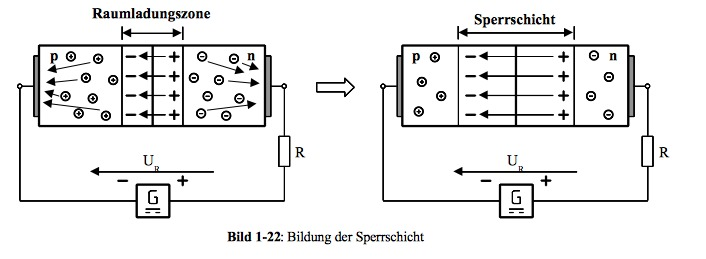
\includegraphics[width=\textwidth]{pnuebergang.jpg}
			  \caption{pn-Übergang einer Diode [gpn]}
			\end{figure}
			
	    \column{.45\textwidth}
	    	\begin{itemize}
	    	  \item Diode: Übergang zwischen n-dotierter zu p-dotierter Schicht
			  \item Ausbilden einer Raumladungszone durch Diffusion der freien Ladungsträger
			  \item Spannung in Sperrrichtung: kein Stromfluss möglich
			\end{itemize}
    \end{columns}
\end{frame}


\begin{frame}{Grundlagen}
    \begin{columns}[T]	
	    \column{.45\textwidth}
	    	\begin{itemize}
	    	  \item eintreffende Strahlung erzeugt $e^-$/Loch-Paare: $e^-$ werden ins Leitungsband
	    	  gehoben, Löcher bleiben im Valenzband zurück
	    	  \item Diffusion der freien $e^-$ zur Anode, Diffusion der Löcher zur Kathode $\rightarrow$
	    	  messbarer Strom $\propto$ Energie des Teilchens
			\end{itemize}
			
		\column{.5\textwidth}
			\begin{figure}[htbp]
			  \centering
			  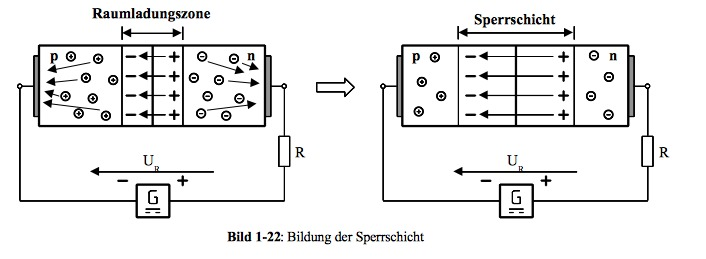
\includegraphics[width=\textwidth]{pnuebergang.jpg}
			  \caption{pn-Übergang einer Diode [gpn]}
			\end{figure}
    \end{columns}
\end{frame}